\scanpage{118}
\deleted{
1. \inserted{Morphismes plats \unsure{etc.}} Changement de base, \deleted{platitude}

2. $\underset{\longleftarrow}{\operatorname{Lim}}$ de préschémas, propriétés constructibles

3. \unsure{(?)} Morphismes réguliers etc. Application à l'algèbre locale.

Pourrait passer au Chap 0 ?

4. Morphismes plats de présentation finie: critères de platitude

5. Immersions régulières etc

6. Dimension, morphismes équidimensionnels

7. Morphismes univ$^t$. ouverts.

8. Calcul diff$^l$. Morphismes diff$^t$ simples.

9. Morphismes simples

10. Morphismes étales, morphismes non ramifiés

11. Fibres d'un morphisme plat de présentation finie. Morphismes séparables, normaux etc

12. Sections hyperplanes, multisections

13. Prolongements infinitésimaux

14. Préschémas de \unsure{Grassm.} Espaces algébriques de Serre.

15. Formes différentielles et dualité
}
\margin{\figure{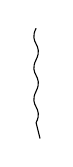
\begin{tikzpicture}
\draw (0,1.4)..controls(-.1,1.2)and(.1,1.2)..(0,1)..controls(-.1,.8)and(.1,.8)..(0,.6)..controls(-.1,.4)and(.1,.4)..(0,.2)--(.05,0);
\end{tikzpicture}}}
\margin{\figure{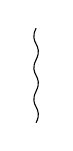
\begin{tikzpicture}
\draw (0,1.2)..controls(-.1,1)and(.1,1)..(0,.8)..controls(-.1,.6)and(.1,.6)..(0,.4)..controls(-.1,.2)and(.1,.2)..(0,0);
\end{tikzpicture}}}
\margin{\figure{\begin{tikzpicture}\draw (.12,2)--(0,2)--(0,0)--(.12,0);\end{tikzpicture}}}
\margin{\figure{
\begin{tikzpicture}
\draw[line width=1pt] (0,1.4)..controls(-.1,1.2)and(.1,1.2)..(0,1)..controls(-.1,.8)and(.1,.8)..(0,.6)..controls(-.1,.4)and(.1,.4)..(0,.2)--(.05,0);
\end{tikzpicture}}}
\margin{\figure{
\begin{tikzpicture}\fill (0,0) rectangle(.1,.7);\end{tikzpicture}}}
\figure{
\begin{tikzpicture}\draw (0,0)--(12,-.05);\end{tikzpicture}}

\deleted{
$*$ \deleted{James September 1963}

$*$ Bott September 1963 ?

$*$ \uline{Zariski} for Dieudonné: \unsure{Give} a talk at the Colloquium of Harvard

$*$ \uline{Hilton} on the mailing list / \unsure{Prog.} II for Kuiper for myself

\deleted{copy of my talks to Baltimore}

$*$ \deleted{Paper by Eells-Kuiper.}
}
\figure{\begin{tikzpicture}
\draw (.2,2.6)--(0,2.6)--(0,1);\draw(.4,1.7)--(2.2,1.7);
\draw(.4,.7)--(2.4,.7);\draw(.4,-.8)--(2.5,-.8);\draw(0,-1.8)--(3,-1.8);
\draw(6.2,.6)--(6.3,-.8)--(6.1,-.8);
\end{tikzpicture}}
\mspage{117}

